\documentclass[a4paper,11pt,DIV=12,overfullrule=on]{scrreprt}%
\usepackage{unicode-math}%
\usepackage{polyglossia}%
\setdefaultlanguage[spelling=new, babelshorthands=true]{german}
\usepackage{fontspec}
\setdefaultlanguage{german}%
\setotherlanguage{english}%
\setmainfont[Mapping=tex-text]{Raleway}%

\setmonofont[Mapping=tex-text, Scale=0.9]{Fira Code Light}%
\setmathfont{Asana Math}%
\newfontface\RalewaySemi{Raleway SemiBold}
\setkomafont{disposition}{\RalewaySemi}
\addtokomafont{subject}{\RalewaySemi}


\usepackage{xltxtra}%
\usepackage{microtype}%
\usepackage[svgnames, x11names, xetex, rgb, RGB, HTML, hyperref]{xcolor}%
\definecolor{shortyblue}{HTML}{1976D2}  % FIXME: Echte Farbwerte eintragen

\definecolor{background}{HTML}{EEEEEE}
\definecolor{eclipseStrings}{RGB}{42,0.0,255}
\definecolor{eclipseKeywords}{RGB}{127,0,85}
\definecolor{mediumgray}{rgb}{0.3, 0.4, 0.4}
\definecolor{mediumblue}{HTML}{079cff}
\definecolor{forestgreen}{rgb}{0.13, 0.55, 0.13}
\definecolor{darkviolet}{rgb}{0.58, 0.0, 0.83}
\definecolor{royalblue}{rgb}{0.25, 0.41, 0.88}
\definecolor{crimson}{rgb}{0.86, 0.8, 0.24}
\colorlet{numb}{magenta!60!black}
\usepackage{listings}
\lstset{%
    abovecaptionskip=\medskipamount,
    aboveskip=\bigskipamount,
    backgroundcolor=\color{background},
    basicstyle=\normalfont\ttfamily,
    breakatwhitespace=false,
    breaklines=true,
    captionpos=b,
    columns=fullflexible,
    commentstyle=\color{eclipseStrings}, % style of comment
    emphstyle=\color{crimson},
    extendedchars=true,  % requires inputenc
    fontadjust=true,
    frame=lines,
    identifierstyle=\color{black},
    keepspaces=true,
    keywordstyle=\bfseries\color{mediumblue},
    keywordstyle={[2]\bfseries\color{darkviolet}},
    keywordstyle={[3]\bfseries\color{royalblue}},
    keywordstyle={[4]\bfseries\color{royalblue}},
    numbers=left,
    numbersep=8pt,
    numberstyle=\scriptsize,
    rulecolor=\color{black},
    showlines=true,
    showspaces=false,
    showstringspaces=false,
    showtabs=true,
    stringstyle=\color{eclipseKeywords}, % style of strings
    tabsize=4,
    title=\lstname,
    xleftmargin={18pt},
}

\lstdefinelanguage{json}{
    string=[s]{"}{"},
    comment=[l]{:\ "},
    morecomment=[l]{:"},
    literate=
        *{0}{{{\color{numb}0}}}{1}
        {1}{{{\color{numb}1}}}{1}
        {2}{{{\color{numb}2}}}{1}
        {3}{{{\color{numb}3}}}{1}
        {4}{{{\color{numb}4}}}{1}
        {5}{{{\color{numb}5}}}{1}
        {6}{{{\color{numb}6}}}{1}
        {7}{{{\color{numb}7}}}{1}
        {8}{{{\color{numb}8}}}{1}
        {9}{{{\color{numb}9}}}{1}
        }
        
\lstdefinelanguage{JavaScript}{
    stringstyle=\color{forestgreen},
    morekeywords=[1]{await, async, case, catch, class, const, default, do,
        enum, export, extends, finally, from, implements, import, instanceof,
        let, static, super, switch, throw, try},
    morekeywords=[2]{break, continue, delete, else, for, function, if, in,
        new, return, this, typeof, var, void, while, with},
    morekeywords=[3]{false, null, true, boolean, number, undefined,
        Array, Boolean, Date, Math, Number, String, Object},
    morekeywords=[4]{eval, parseInt, parseFloat, escape, unescape},
        sensitive,
    morecomment=[s]{/*}{*/},
    morecomment=[l]//,
    morecomment=[s]{/**}{*/},
    morestring=[b]',
    morestring=[b]",
    morestring=[b]`
}[keywords, comments, strings]





\usepackage[xetex, hyperindex, pdfpagelabels]{hyperref}
\hypersetup{
    pdfauthor = {Markus Rennings, Deniz Durmaz},
    pdftitle = {Shorty – URL-Shortener, Gruppe 3, Projektphase 2},
    pdfsubject = {Projektdokumentation Shorty},
    pdfkeywords = {Projekt, Projektphase, aws2302, Shorty, URL-Shortener},
    pdfcreator = {XeLaTeX with hyperref package},
    pdfproducer = {pdfLaTeX},
    pdfdisplaydoctitle = {true},
    pdfduplex = {DuplexFlipLongEdge},
    pdfnewwindow = {true},
    colorlinks = true,
    linkcolor = shortyblue,          % color of internal links
    citecolor = green,        % color of links to bibliography
    filecolor = magenta,      % color of file links
    urlcolor = shortyblue,          % color of external links
    breaklinks = true
}
\usepackage{graphicx}
\graphicspath{ {img/} }%
\usepackage{acronym}%


% Title Page
\subject{Projekt 2, Gruppe 3}
\title{Shorty – URL-Shortener}
\subtitle{}
\author{Andreas Brühl\thanks{Datenbank} \and Deniz Durmaz\thanks{Design, Frontend, Dokumentation} \and Sebastian Hufeld\thanks{Design, Datenbank, DB-Dokumentation} \and Jason Krimmel\thanks{Design, Frontend} \and Markus Rennings\thanks{API-Design, Backend, OpenAPI, Dokumentation, \XeLaTeX}}
\date{23.\,August–5.\,September~2023}
\publishers{Betreut durch: Martin Dubb, Fabio Keller}


\begin{document}
%\raggedbottom%
\maketitle

\tableofcontents

% ! 1. Einleitung
\chapter{Einleitung}
\section{Kontext der Arbeit}
Das Projekt wurde im Rahmen einer geförderten Weiterbildung erstellt. Der Träger der Weiterbildung ist die Techstarter GmbH\footnote{\href{https://techstarter.de/}{https://techstarter.de/}}. Es gab mehrere Projekte zur Auswahl mit freier Gruppen- und Themenfindung. Das gewählte Projekt ist ein URL Shortener.

\section{Motivation für diese Arbeit}
In der Weiterbildung wurden verschiedene Methoden und Themenbereiche vermittelt. Diese sollen und werden in diesem Full-Stack-Projekt zusammengeführt und genutzt. So soll zum einen gezeigt werden, wie wir diese vielen Teilbereiche nutzen, um das Projekt umzusetzen.

Die größte Problematik ist es, sich erst einmal als Gruppe zu finden, aufzuteilen und zu sortieren, um die Anforderungen umzusetzen.

\section{Zielstellung für diese Arbeit}
Unsere Lösung wandelt lange \ac{URL} in kurze und eindeutige \ac{URL}s um. Bei \ac{URL}s kann die Zeichenlänge je nach Darstellung in mehreren Zeilen ausarten. Das kann zu Problemen in Dokumenten, E-Mails oder Social-Media-Posts führen. Durch die gekürzten \ac{URL}s wird dieses Problem behoben oder aber auch, wenn eine Zeichenbegrenzung vorhanden ist, wird diese nicht durch die lange \ac{URL} kannibalisiert. Optisch sind Short-\ac{URL}s ebenfalls nicht so aufdringlich.

\section{Anforderungen für diese Arbeit}
\begin{description}
    \item[URL-Validierung] Es ist erforderlich, eine \ac{URL}-Validierung zu implementieren, um sicherzustellen, dass die eingegebenen \ac{URL}s gültig sind.
    \item[URL-Kürzung] Die Lösung muss in der Lage sein, lange \ac{URL}s in kurze \ac{URL}s umzuwandeln.
    \item[Generierung von Kurzlink-Codes] Die Kurzlinks müssen eindeutig sein.
    \item[Benutzeroberfläche] Es muss eine benutzerfreundliche Oberfläche sein, über die Nutzer \ac{URL}s eingeben und Kurzlinks generieren können.
    \item[Anzeige von Kurzlinks] Benutzer bekommen bei Generierung des Kurz-Links ein Passwort mitgeteilt, mit dem sie sich die Statistik zu dem Link anschauen können. Diese Statistik umfasst eine Auswertung, wie oft auf den Link zugegriffen wurde, mit welchen Browsers und mit welchem \ac{OS}. Auch der Zeitpunkt des letzten Zugriffs wird ausgewertet.
    \item[Datenbank] Die Anwendung muss die ursprünglichen \ac{URL}s und die zugehörigen Kurzlinks in einer Datenbank speichern und die Verknüpfung zwischen ihnen sicherstellen.
    \item[API] Ein \ac{API} muss entwickelt werden, um die Interaktion zwischen Frontend und Backend zu ermöglichen. Dies ermöglicht das Erstellen und das Abrufen von Kurzlinks. Das gleiche gilt für die dazugehörigen Statistiken.
    \item[Statistik und Analyse] Die Anwendung muss die Daten über die Nutzung der generierten Kurzlinks sammeln und speichern. Einschließlich Anzahl der Klicks, Zeitpunkt der Nutzung und Informationen zu \ac{OS} und Browser der Nutzer, müssen generiert werden.
    \item[Passwortschutz für Link-Bearbeitung und Statistik] Jeder generierte Kurzlink muss über ein eindeutiges Schlüssel/Passwort verfügen, mit dem Benutzer den Link bearbeiten und die Statistiken einsehen können.
    \item[Programmiersprache] Als Programmiersprache wurde \ac{JS} vorgegeben. Es durften Bibliotheken verwendet werden.
\end{description}

% ! 2. Technische Grundlagen
\chapter{Technische Grundlagen}
Grundsätzlich sind weitläufige Kenntnisse aus der Webentwicklung erforderlich, um die Architektur und die Komponenten des Full-Stack-Projekt umzusetzen und zu verstehen.

\begin{description}
    \item[Frontend- und Backend-Technologien] Grundlegende Kenntnisse über die Technologien, die im Frontend und Backend verwendet werden, wie z.\,B. \ac{JS} oder \mbox{react.js}, um die Benutzeroberfläche und die Serverseite zu entwickeln und gestalten.

    \item[Datenbank] Verständnis von Datenbankkonzepten und -operationen, insbesondere der Speicherung und Abfrage von Daten.

    \item[API] Schnittstellen-Bildung und Integration zur Sicherstellung einer fehlerfreien Kommunikation zwischen den einzelnen Elementen.

    \item[Sicherheit] Sichere Speicherung von gestellten Anfragen, Benutzern und Passwörtern.

    \item[Statistik und Daten] Speicherung, Abruf und Visualisierung der vorhanden bzw.\ angefragten Daten (\ac{URL}, Klicks) für die Erstellung der Statistik.
\end{description}

\section{Benutzeroberfläche}
\section{Datenbank}
Als Datenbank haben wir uns zum Schluss für eine SQLite3 Datenbank entschieden. Eigentlich war das Projekt mit einer Firebase Datenbank geplant, jedoch gab es bei unserer Implementierung einige Fehler, welche wir leider nicht innerhalb des Projektzeitraums beheben konnten. So haben wir uns schließlich dazu entschlossen, statt einer Online-Datenbank auf eine Offline-Datenbank zu switchen.

Dabei haben wir Firebase nicht gänzlich verworfen und sollte es eine Version 2.0 geben, so ist geplant dort dann auf den Firestore zu wechseln, sodass eine Online-Version der Datenbank zur Verfügung steht.

Die \texttt{url.db} sowie die \texttt{database.js} wurden unter folgendem Pfad gespeichert:

\texttt{server/src/db/url.db}


Dies wurde als genereller Speicherort für die Arbeiten der Datenbank ausgewählt.


Erklärung der einzelnen Felder, welche beim erstellen der Datenbank erstellt werden:

\begin{description}
    \item[longURL] hier wird die Ausgangs-URL hinterlegt
    \item[shortURL] enthält die gekürzte URL
    \item[browser\_*] Anzahl der Aufrufe über einen bestimmten Browser
    \item[os\_*] Anzahl der Aufrufe über ein bestimmtes OS
    \item[lastClick] Zeitpunkt des letzten Aufrufs der shortURL
    \item[clicks] Anzahl der Clicks der jeweiligen ShortURL
    \item[timestamp] Zeitpunkt zu dem der Link/Datenbankeintrag erstellt wurde.
    \item[expireDate] Datum wann der Link erlischt (90 Tage nach Erstellung)
\end{description}

\subsection{Datenbank-Struktur}
Die Datenbank ist wie bereits erwähnt eine SQLite3 Datenbank. Das Schema für diese Datenbank haben wir zusammen erarbeitet (siehe Zeile 4 bis 20 in Lst.~\ref{lst:dbCreate}). In unserem Code wird als erstes überprüft, ob die Datenbank bereits existiert. Sollte dies nicht der Fall sein, so wird diese über die dritte Zeile im Code unter Lst.~\ref{lst:dbCreate} erstellt. 

\subsection{Erstellen der Datenbank}
Als Defaultwert werden für die Browser- und OS-Daten sowie für \texttt{clicks} und \texttt{lastClick} \texttt{0} verwendet. Diese haben wir initial gesetzt, da nach dem Erstellen des Links ja noch keinerlei Informationen vorhanden sind.

\begin{lstlisting}[language=JavaScript,
    caption={Die Statistiken werden initial auf 0 gesetzt, der Timestamp ist der Datumswert der Erstellung des Eintrags},
    label={lst:dbCreate},
    float=h,
    gobble=4
]
    db.serialize(() => {
        db.run(`
            CREATE TABLE IF NOT EXISTS url (
                id INTEGER PRIMARY KEY AUTOINCREMENT,
                longURL TEXT NOT NULL,
                shortURL TEXT NOT NULL,
                passwd TEXT NOT NULL,
                browser_chrome INTEGER NOT NULL default 0,
                browser_firefox INTEGER NOT NULL default 0,
                browser_edge INTEGER NOT NULL default 0,
                browser_safari INTEGER NOT NULL default 0,
                browser_opera INTEGER NOT NULL default 0,
                browser_sonstige INTEGER NOT NULL default 0,
                os_win INTEGER NOT NULL default 0,
                os_mac INTEGER NOT NULL default 0,
                os_linux INTEGER NOT NULL default 0,
                lastClick INTEGER NOT NULL default 0,
                clicks INTEGER NOT NULL default 0,
                timestamp INTEGER,
                expireDate INTEGER
            )
        `);
    });
\end{lstlisting}

\subsubsection{Speichern des Links in der Datenbank}
Nun geht es darum, dass wir den Link auch entsprechend mit allen Informationen in der Datenbank speichern. In Lst.~\ref{lst:dbSave} sieht man dazu die entsprechende Logik. 
In Zeile 2 und 3 werden die jeweiligen Zeitstempel gesetzt. \texttt{currentTime} setzt dabei den Zeitstempel beim erstellen des Link. Das \texttt{expireDate} haben wir anschließend auf 90 Tage gesetzt. Die Formel »\texttt{currentTime + 90 * 24 * 60 * 60 * 1000}« berechnet dabei genau diesen Zeitraum.

Danach werden in der Zeile 6 des Codes die Daten für \texttt{longURL}, \texttt{shortURL}, \texttt{passwd} und der bereits erwähnte Zeitstempel sowie das Verfallsdatum des Links in die Datenbank geschrieben. Die Daten für \texttt{longURL}, \texttt{shortURL} \& \texttt{passwd} werden uns dabei von der API übermittelt.
Wie wir in Lst.~\ref{lst:dbCreate} ja schon gesehen haben, werden alle anderen Werte, welche hier nicht aufgezählt sind, mit \texttt{0} gesetzt. 

Sollte es ein Problem beim Speichern der Daten in die Datenbank geben, so wird dieser Fehler in den Zeilen 10 bis 12 ausgegeben. Wenn hingegen kein Fehler auftritt, so wird die zuletzt erstellte ID für den Eintrag zurückgegeben. 

\begin{lstlisting}[language=JavaScript,
    caption={Speichern der URL in der Datenbank},
    label={lst:dbSave},
    float=h,
    gobble=4
]
    const saveURL = async (result) => {
        const currentTime = Date.now();
        const expireDate = currentTime + 90 * 24 * 60 * 60 * 1000; 
        return new Promise((resolve, reject) => {
            db.run(
                'INSERT INTO url (longURL, shortURL, passwd, timestamp, expireDate) VALUES (?, ?, ?, ?, ?)',
                [result.longUrl, result.shortUrl, result.passwd, currentTime, expireDate],
                function (err) {
                    if (err) {
                        reject(err);
                    } else {
                        resolve(this.lastID);
                    }
                }
            );
        });
    };
\end{lstlisting}

\subsubsection{Statistiken auslesen und an die API übergeben}
Damit die entsprechenden Daten aus der Datenbank über die \texttt{/api/stats}-Route abgerufen werden können, haben wir die Logik in Lst.~\ref{lst:dbAbruf} geschrieben. 
Diese ruft in Zeile 3 alle Informationen zu einem Kurzlink auf. Mit »\texttt{'SELECT * FROM url WHERE shortURL = ?', [shortURL]}« übergeben wir der Datenbank den entsprechenden Link. Die Datenbank gibt uns anschließend alle Infos zurück, die zu dem gespeicherten Link vorhanden sind. 

Sollte es einen Fehler geben, so wird dieser wieder ausgeworfen. Dies passiert in Zeile 4 \& 5. Sollte es hingegen keinen Fehler geben, greift der \texttt{else} Zweig und gibt uns die entsprechende Spalte der Tabelle aus. 

\begin{lstlisting}[language=JavaScript,
    caption={Daten werden von der Datenbank anhand des Kurzlinks abgerufen},
    label={lst:dbAbruf},
    float=h,
    gobble=4
]
    const getStats = async (shortURL) => {
        return new Promise((resolve, reject) => {
            db.get('SELECT * FROM url WHERE shortURL = ?', [shortURL], (err, row) => {
                if (err) {
                    reject(err);
                } else {
                    resolve(row);
                }
            });
        });
    };
\end{lstlisting}

\subsubsection{Update der Statistikdaten in der Datenbank mit den Infos von der API}
Um die Daten entsprechend zu aktualisieren, haben wir die Logik in Lst.~\ref{lst:dbUpdate} geschrieben. Mit dem »\texttt{Update}« Befehl in Zeile 4 aktualisieren wir in unserer Datenbank die Daten, die wir von der API bekommen. Dabei werden die jeweiligen Statistiken für die aufgezählten Browser (Zeilen 8 bis 13), das entsprechende Betriebssystem (Zeilen 14 bis 16) sowie der letzte Klick (Zeile 17) und die generellen Clicks (Zeile 18).

Auch hier haben wir wieder das Fehlerhandling so gebaut, dass er bei Fehler die entsprechende Fehlermeldung auswirft und bei keiner Fehlermeldung die Daten in die Datenbank schreibt (Zeile 21 bis 25).

\begin{lstlisting}[language=JavaScript,
    caption={Die Daten werden von der API an uns übermittelt und wir speichern die Daten in der Datenbank beim entsprechenden Kurzlink ab},
    label={lst:dbUpdate},
    float=h,
    gobble=4
]
    const writeStats = (shortURL, stats) => {
        return new Promise((resolve, reject) => {
            db.run(
                'UPDATE url SET browser_chrome = ?, browser_firefox = ?, browser_edge = ?, browser_safari = ?, browser_opera = ?, browser_sonstige = ?, os_win = ?, os_mac = ?, os_linux = ?, lastClick = ?, clicks = ? WHERE shortURL = ?',
                [
                    stats.Browser.Chrome,
                    stats.Browser.Firefox,
                    stats.Browser.Edge,
                    stats.Browser.Safari,
                    stats.Browser.Opera,
                    stats.Browser.Sonstige,
                    stats.OS.Windows,
                    stats.OS.MacOs,
                    stats.OS.Linux,
                    stats.lastClick,
                    stats.clicks,
                    shortURL,
                ],
                (err) => {
                    if (err) {
                        reject(err);
                    } else {
                        resolve();
                    }
                }
            );
        });
    };
\end{lstlisting}

\section{Statistik und Analyse}
Für die Statistik nutzen wir die Express.js-Middleware \texttt{express-useragent}\footnote{\href{https://www.npmjs.com/package/express-useragent}{https://www.npmjs.com/package/express-useragent}}, welches die User-Agent-Kennungen zusammenfasst, so dass man nicht für jede Browser-Version einzeln checken muss. Diese Daten werden in der Datenbank kumuliert und bei Anfrage entsprechend über den \ac{API}-Endpunkt \texttt{/api/stats/\{shortUrl\}} an den Client gesendet. Die Statistiken sind mit einem Passwort geschützt, dass dem Benutzer bei Erstellung der Kurz-URL angezeigt wird.

\section{API}
Die \ac{API} bietet verschiedene Endpunkte für den Zugriff. So wird zur Erstellung eines Kurz-Links der http-POST-Endpunkt »\texttt{/}« genutzt, zur Weiterleitung (Abfrage des Kurz-Links) wird der Endpunkt »\texttt{/\{shorturl\}}« verwendet. Und zur Abfrage der Statistiken dient der POST-Endpunkt »\texttt{/api/stats/\{shortUrl\}}«. 
\section{URL-Validierung}
Zur Validierung der URL nutzen wir das Paket \texttt{url-http}\footnote{\href{https://www.npmjs.com/package/url-http}{https://www.npmjs.com/package/url-http}} mit einer kleinen Wrapper-Funktion (siehe Lst.~\ref{lst:wrapperUrlVal}), wobei die \ac{URL} inklusive Schema (\texttt{http://} bzw. \texttt{https://}) erwartet wird.

\begin{lstlisting}[language=JavaScript,
    caption={Wrapper-Funktion zur URL-Validierung},
    label={lst:wrapperUrlVal},
    float=h,
    gobble=4
]
    const isValidUrl = (url) => !!httpUrl(url);
\end{lstlisting}

% \begin{figure}[h]%
%     \begin{small}%
%         \begin{center}%
%             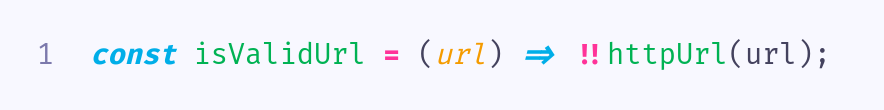
\includegraphics[width=0.8\textwidth]{2_5_wrapper.png}%
%         \end{center}%
%         \caption{Quelltextauschnitt der Wrapper-Funktion zur \ac{URL}-Validierung}%
%         \label{fig:25wrapper}%
%     \end{small}%
% \end{figure}%

\section{URL-Kürzung}
Die eigentliche URL-Kürzung entsteht durch einen Datenbank-Eintrag, der die generierte Kurz-\ac{URL} (ID) mit der langen \ac{URL} verknüpft und zusätzlich die statistischen Daten zu jedem Kurzlink speichert.
\subsection{Algorithmus}
Wir haben uns für die Verwendung eines 58-stelligen Alphabets (Base-58\label{sec:base58}, siehe Lst.~\ref{lst:base58}, Zeile~1) für die Generierung der ID entschieden. Hierzu werden von einem Base62-Alphabet (\texttt{[0–9A–Za–z]}) die Zeichen »0« (Null), »I« (Großbuchstabe i), »O« (Großbuchstabe o) und »l« (Kleinbuchstabe L) entfernt, da diese – je nach Schriftart – verwechselt werden können. Hierdurch wird zwar die Anzahl der möglichen IDs eingeschränkt, aber $58^7 =  2\,207\,984\,167\,552$ Möglichkeiten sollten diese immer noch ausreichen.

Die eigentliche Kurz-\ac{URL} ist dann ein siebenstelliger base58-kodierter String aus einer Kombination aus Teilen des Unix-Zeitstempels (Lst.~\ref{lst:shorturl} Zeilen 1–3) und einer zweistelligen Zufallszahl (Zeile 4). Zum einfacheren Verbinden beider Zahlen werden diese zunächst als String generiert und erst bei Übergabe an die Funktion \texttt{base58()} als Integer umgewandelt (ebenfalls Zeile 4 in Lst.~\ref{lst:shorturl}).

\begin{lstlisting}[language=JavaScript,
    caption={Aufbau der Basis vor der base58-Konvertierung},
    label={lst:shorturl},
    float=h,
    gobble=4
]
    let date = Date.now()
        .toString()
        .slice(1,-2);
    const shortUrl = base58(parseInt(getRnd() + date));
\end{lstlisting}

% \begin{figure}[h]%
%     \begin{small}%
%         \begin{center}%
%             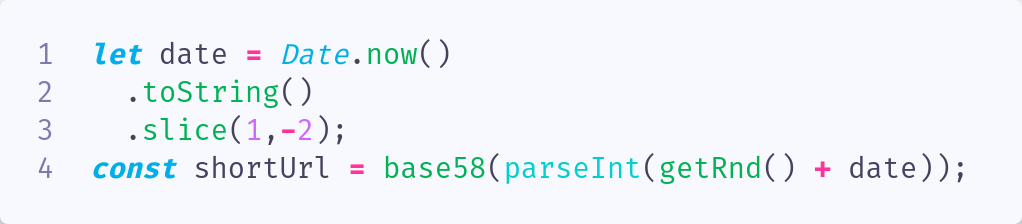
\includegraphics[width=0.8\textwidth]{2_6_1_shortUrl.png}%
%         \end{center}%
%         \caption{Quelltextauschnitt zur Generierung der Kurz-Url}%
%         \label{fig:261shorturl}%
%     \end{small}%
% \end{figure}%


\section{Passwort für Link-Bearbeitung und Statistik}
Das Passwort für die generierte Kurz-\ac{URL} lassen wir uns als zufällige, zwölfstellige alphanumerische Zeichenkette durch das Modul »generate-password«\footnote{\href{https://www.npmjs.com/package/generate-password}{https://www.npmjs.com/package/generate-password}} erstellen.


% ! 3. Beschreibung der Lösung
\chapter{Beschreibung der Lösung}
\section{Software-Architektur der Lösung}
\section{Übersicht und Zusammenspiel der Komponenten}
\section{Beschreibung der Komponenten}
\subsection{Backend}
Wie bereits in Kapitel \ref{sec:base58} beschrieben, haben wir uns für eine \texttt{base58}-Kodierung der Kurz-\ac{URL}s entschieden. Hierzu wurde das entsprechene Alphabet definiert (siehe Lst.~\ref{lst:base58}, Zeile 1). Nach einem Check, ob es eine Ganzzahl $< 0$ ist (Zeilen 4–8), wird innerhalb der \texttt{while}-Schleife (ab Zeile 11, Lst.~\ref{lst:base58}) dann nach dem Restwertverfahren die Eingabezahl konvertiert.

Zwar wäre diese Umrechnung auch wieder umkehrbar (bijektiv), aber da es eine generierte Zahl ist, die keine Verbindung mit der zu kürzenden \ac{URL} hat, verzichten wir darauf und nehmen zur Identifikation die \texttt{base58}-kodierte Zahl als Schlüssel.

Aufgrund der in Lst.~\ref{lst:shorturl} gezeigten Generierung der Ausgangszahl, kann es unter seltenen Umständen dazu kommen, dass bei mehreren gleichzeitigen Zugriffen auch die gleiche Zufallszahl generiert wird. Dazu müsste allerdings in der gleichen Zehntelsekunde auch noch die gleiche Zufallszahl durch \texttt{getRnd()} erzeugt werden. Auch wenn dies nicht komplett ausgeschlossen werden kann, haben wir uns dazu entschieden, dies zu vernachlässigen. Diesen Fall kann man – in einer späteren Erweiterung (siehe auch Kapitel~\ref{sec:ErweiterungKollision}) – auch durch eine Datenbankabfrage und evtl. Neugenerierung der Zufalls-ID umgehen.

\begin{lstlisting}[
    language=JavaScript,
    caption={base58-Konvertierung},
    label={lst:base58},
    float=h,
    gobble=4
]
    const CHARS58 = '123456789ABCDEFGHJKLMNPQRSTUVWXYZabcdefghijkmnopqrstuvwxyz';

    function encode(num) {
        if (isNaN(num) || num % 1 !== 0 || num < 0) {
            // Keine Zahl, oder Float, oder < 0
            return false;
        } else if (num === 0) {
            return '0';
        } else {
            let id = '';
            while (num > 0) {
            id = CHARS58[(num % 58)] + id;
            num = Math.floor(num / 58);
            }
            return id;
        }
    }
\end{lstlisting}


\subsubsection{Schnittstellen der Komponente}
Es gibt drei Schnittstellen der \ac{API}:
\begin{description}
    \item[/] POST-Endpunkt, um eine neue Kurz-\ac{URL} zu generieren
    \item[/\{shortUrl\}] Endpunkt für alle HTTP-Methoden, um eine Kurz-\ac{URL} abzurufen. Der Abrufende wird automatisch, mittels http-Status 307, an die Zieladresse weitergeleitet.
    \item[/api/stats/\{shortUrl\}] POST-Endpunkt zum Abruf der Statistik zu der angegebenen Kurz-\ac{URL}. Das Passwort muss im Request-Body gesendet werden.
\end{description}
Für eine genaue (technische) Dokumentation haben wir die \ac{API}-Dokumentation im OpenAPI-Format\footnote{\href{https://swagger.io/specification/}{https://swagger.io/specification/}} erstellt, welche über das Backend\footnote{\href{http://localhost:8080/api/doc/api}{Backend:Port/api/doc/api}} abrufbar ist.
\subsubsection{Weiterleitung}
Wir leiten mit dem HTTP-Status-Code »307« weiter, so dass sichergestellt ist, dass der Client seine Anfrage mit der gleichen HTTP-Methode an den Server stellt, auf den die Short-\ac{URL} referenziert.
\subsubsection{Datenstrukturen}
Die Daten werden in einer Document-Database (Google Firebase Firestorm\footnote{\href{https://firebase.google.com/}{https://firebase.google.com/}}) gespeichert, und können im \ac{JSON}-Format abgerufen und geschrieben werden.

Wir haben uns für eine recht einfache Struktur entschieden, siehe Lst.~\ref{lst:struktur}.
\begin{lstlisting}[language=json,
    float=h,
    caption={Aufbau der Datenstruktur für jede Kurz-Url},
    label={lst:struktur}]
{
    "clicks": 0,
    "lastClick": timestamp,
    "OS": {
        "Linux": 0,
        "Windows": 0,
        "MacOs": 0,
    },
    "Browser": {
        "Chrome": 0,
        "Edge": 0,
        "Firefox": 0,
        "Opera": 0,
        "Safari": 0,
        "Sonstige": 0,
    },
    "createDate": timestamp,
    "expireDate": timestamp,
    "longURL": "http://ex.amp.le/",
    "shortURL": "aB1Cd2e",
    "Password": "password"
}
\end{lstlisting}
\subsubsection{Funktionsweise}
\subsection{Frontend}
\subsubsection{Sub-Komponente 1}
\paragraph{Aufgabe der Komponente}
\paragraph{Schnittstellen der Komponente}
\subsubsection{Sub-Komponente 2}
\section{Übersicht Verzeichnisse und Dateien}
Auf Top-Level wurde für jede Komponente ein Verzeichnis erstellt. Innerhalb dieser wurde von den jeweiligen Teams eine eigene Struktur etabliert.

\subsection{Backend}
Im Backend \texttt{/server} wurde für die \ac{API}-Endpunkte das Verzeichnis \texttt{api/} erstellt, welches wiederum die Unterverzeichnisse \texttt{doc/} und \texttt{stats/} enthält, welche die jeweiligen Pfade der Endpunkte abbilden.

Im Verzeichnis \texttt{src/} im \texttt{/server}-Verzeichnis befinden sich \ac{JS}-Dateien, die Funktionen für die Endpunkte bereitstellen, z.\,B. die \texttt{base58()}-Kodierung. Unterhalb des \texttt{src}"=Verzeichnisses liegen die Datenbank-Funktionen in ihrem \texttt{db}-Verzeichnis.

Der Einstiegspunkt für das Backend liegt \texttt{/server/index.js}.

\subsection{Frontend}

\subsection{Dokumentation}
Da die Dokumentation das komplette Projekt, mit allen (Sub"~)""Komponenten umfasst, hat diese ihr eigenes (projektbezogenes) Top-Level-Verzeichnis: \texttt{/Dokumentation}. Hier befinden sich sowohl die \texttt{.tex}-Dateien, als auch die \texttt{.yaml}-Datei der OpenAPI-Dokumentation.
\subsection{Struktur}
Daraus ergibt sich dann folgende Verzeichnisstruktur:
\begin{verbatim}
    .
    ├── Dokumentation
    ├── frontend
    │   ├── public
    │   └── src
    │       ├── components
    │       │   └── css
    │       └── pages
    └── server
        ├── api
        │   ├── doc
        │   ├── stats
        ├── controller
        └── src
            └── db
    
\end{verbatim}

\section{Bauen des Gesamtsystems}
Ist dies nicht Kapitel 4.1?


% ! 4. Einrichtung und Betrieb der Software-Lösung
\chapter{Einrichtung und Betrieb der Software-Lösung}
\section{Inbetriebnahme der Lösung}
\section{Möglichkeiten zur späteren Anpassung und Weiterentwicklung}
Es bestehen diverse Möglichkeiten, das Projekt weiterzuentwickeln:
\begin{itemize}
    \item Die Statistiken können erweitert werden, so dass man auch nach mobilen (Smartphone, Tablet) oder stationären (Desktop/Laptop, Smart-TV) auswerten kann.
    \item Auch können die \ac{API}-Endpunkte erweitert werden, so dass z.\,B. nur Werte zu einer bestimmten Statistik abgerufen werden können.
    \item Es kann auch dahingehend erweitert werden, dass sich Benutzer registrieren und anmelden können. Dann kann auch für den eingeloggten Nutzer ein Verlauf der generierten Kurz-\ac{URL}s angezeigt werden und die jeweiligen Statistiken mit einem einfachen Button aufrufbar gemacht werden.
    \item Es kann ein DELETE-Endpunkt implementiert werden, damit ein Benutzer seinen generierten Link vorzeitig löschen kann.
    \item Die generierten Links sollten auch nach einer voreingestellten Zeit automatisch gelöscht werden. Diese Zeit kann bis zu einer Obergrenze von Nutzer festgelegt werden. Das Löschen selbst kann beispielsweise durch einen Endpunkt erfolgen, der von außen mitteln {\ttfamily cron} und {\ttfamily curl} angesprochen wird. Das Feld {\ttfamily expireDate} ist schon in jedem Datensatz enthalten und wird standardmäßig auf Erstellungszeit $+$ 30 Tage gesetzt.
    \item \label{sec:ErweiterungKollision}Es kann (sollte?) eine Sicherheitsabfrage eingebaut werden, die das Erzeugen – und damit das Überschreiben – identischer Kurz-IDs unterbindet.
    \item Zum Einsatz »in production« sollten auf jeden Fall noch die Benutzereingaben auf Vollständigkeit und Schadcode überprüft werden.
    \item Ebenfalls für den produktiven Einsatz können entsprechende Log-Meldungen eingepflegt werden. Hierzu kann auch die Logging-Bibliothek geändert werden, z.\,B. zu »Winston«\footnote{\href{https://github.com/winstonjs/winston}{https://github.com/winstonjs/winston}}.
\end{itemize}
    
% ! 5. Retrospektive
\chapter{Retrospektive}
\section{Evaluierung der Projektergebnisse}
\section{Bewertung der eigenen Arbeitsweise und die Zusammenarbeit im Team}
\section{Gewonnene Erkenntnisse für zukünftige Projekte}

% ! 6. Zusammenfassung und Ausblick
\chapter{Zusammenfassung und Ausblick}

\chapter*{Liste der Abkürzungen}
\begin{acronym}
    \acro{API}{Application Programming Interface (Programmierschnittstelle)}
    \acro{JS}{Javascript}
    \acro{JSON}{Javascript Object Notation}
    \acro{OS}{Operating System (Betriebssystem)}
    \acro{URL}{Uniform Resource Locator}
\end{acronym}

%\listoftables
%\listoffigures
\lstlistoflistings
\end{document}
